\chapter{K-means Clustering Algorithm}
\section{Background}
Even though K-means was first proposed over fifty years ago, it is still one of the most widely used algorithms for clustering. Ease of implementation, simplicity, efficiency, and empirical success are the main reasons for its popularity.
The main features of the conventional K-means clustering algorithm \cite{hartigan} are as follows.
\begin{enumerate}
\item It is a partitional or non-hierarchical clustering method.
\item The total number of clusters, k, is assumed to be fixed and known before hand.
\item It uses Euclidean distance as the criterion for finding distance between the data points and hence, is only applicable to numerical data.
\item It is a greedy iterative method and the iterations continue till the error function has not reached a threshold or the membership of the data points no longer changes.
\end{enumerate}

\section{Algorithm}\label{sec:names}

Let $D = \lbrace x_{i}, i = 1,...,n \rbrace$ be the given input data set of $d$ dimensional data points. Let $K$ be the total number of disjoint clusters, denoted by $C = \lbrace c_{k}, k = 1,...,K\rbrace$. For each cluster $c_{k}$ let $\mu\left( c_{k}\right) $ be its centroid or mean. Then the error function is defined as $$E\left( C\right) = \sum_{k=1}^{K}{\sum_{x\epsilon c_{k}}^{}{\Vert x - \mu\left( c_{k}\right)\Vert^{2} }}$$
The aim of K-means is to minimize the value of the error function $E\left(C)\right)$ which is an NP-hard problem \cite{drineas}.

The pseudo code for conventional K-means algorithm is shown in Algorithm \ref{algo:kmean}. 
\begin{algorithm} 
\caption{\textsc{K-means Algorithm}}
\label{algo:kmean}
\begin{algorithmic}[1]
\REQUIRE Dataset $D$ containing $n$ $d$-dimensional points, Number of clusters $K$, Error threshold $E_{t}$
\ENSURE $K$ disjoint clusters, $C = \lbrace c_{k}, k = 1,...,K\rbrace$ with their members.
%\STATE Initialization()
\STATE $\lbrace c_{1},c_{2},...,c_{k}\rbrace$ be the initial $K$ partitions.\label{algo:kmean:init}
\REPEAT
%\STATE FindNearest()
\FORALL{data-point $x$ in $D$} \label{algo:kmean:nearest}
	\STATE Let $x$ belongs to cluster $c_{1}$.
	\STATE $min_{dist} \gets \Vert x - \mu \left(c_{1}\right)\Vert^{2}$
	\FORALL{centroid $\mu$}
		\STATE $dist \gets \Vert x - \mu\Vert^{2}$
		\STATE If $dist < min_{dist}$, assign $x$ to $\mu$
	\ENDFOR
\ENDFOR
%\STATE Compute()
\STATE Recompute the cluster centroids based on above assignments. \label{algo:kmean:compute}
\STATE Calculate the error function $E\left(C\right)$.
\UNTIL either there were no changes in cluster membership or value of $E\left(C\right) < E_{t}$. \label{algo:kmean:term}
\end{algorithmic}
\end{algorithm}


\section{Analysis}
K-means algorithm tries to terminate at a local optimum. It always converges to a local minimum point \cite{selim} after a finite number of iterations and so the value of error function $E\left(C\right)$ is always non-increasing.
The most important choice for K-means algorithm is the choice of value $K$. Also, the final set of clusters and the number of iterations taken to reach them is dependent on the initially selected centroids (Step \ref{algo:kmean:init} in Algorithm \ref{algo:kmean}). Figure \ref{fig:kmean} illustrates the execution of K-means Algorithm \ref{algo:kmean}.

\begin{figure}[h]
	\centerline{
   \subfloat[Initial Phase]{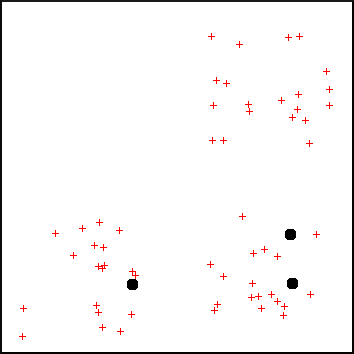
\includegraphics[width=0.3\textwidth]{./Data/kmeans_algo/initial}  	\label{fig:kmean_init} }
   \subfloat[$1^{st}$ Assignment]{	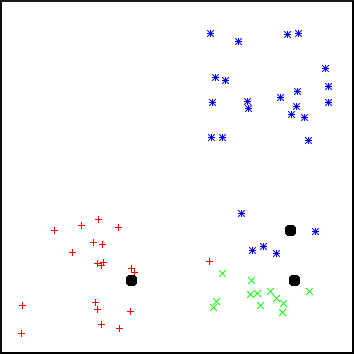
\includegraphics[width=0.3\textwidth]{./Data/kmeans_algo/first_assign}  	\label{fig:kmean_assign1} }
   \subfloat[$1^{st}$ Re-computation]{	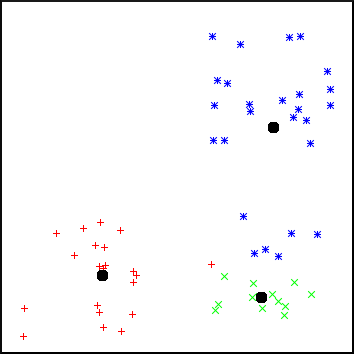
\includegraphics[width=0.3\textwidth]{./Data/kmeans_algo/first_compute}  	\label{fig:kmean_compute1} }
   }

	\centerline{
   \subfloat[$2^{nd}$ Assignment]{	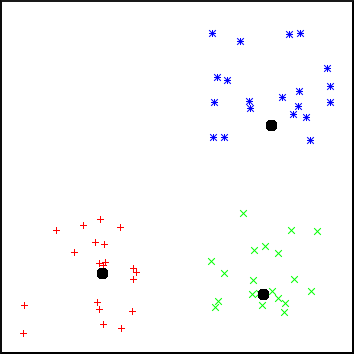
\includegraphics[width=0.3\textwidth]{./Data/kmeans_algo/second_assign}  	\label{fig:kmean_assign2} }
   \subfloat[$2^{nd}$ Re-computation]{	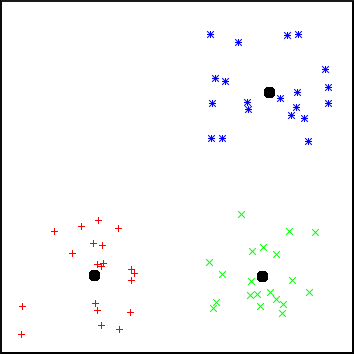
\includegraphics[width=0.3\textwidth]{./Data/kmeans_algo/second_compute}  	\label{fig:kmean_compute2} }
   \subfloat[Final Assignment]{	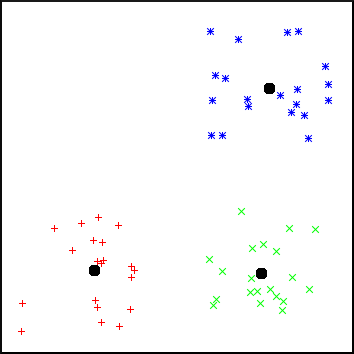
\includegraphics[width=0.3\textwidth]{./Data/kmeans_algo/third_assign}  	\label{fig:kmean_assign3} }
	}
	\caption{Illustration of the K-means Algorithm \ref{algo:kmean} for two-dimensional data points when number of clusters, $K = 3$}
\label{fig:kmean}
\end{figure}

We consider the case where the input data points are two-dimensional and the value of $K$ is 3. Figure \ref{fig:kmean_init} shows the initialization phase (Step \ref{algo:kmean:init}) of the algorithm. Three random data-points have been selected as the initial centroids. In the first iteration, the assignment stage (Step \ref{algo:kmean:nearest}) assigns the data points to the initial centroids based on their Euclidean distance with the initially selected centroids as depicted in Figure \ref{fig:kmean_assign1}. In the re-computation stage, (Step \ref{algo:kmean:compute}) the centroids are re-computed to their new values (Figure \ref{fig:kmean_compute1}).

In the second iteration, during assignment of data points many points change their cluster (Figure \ref{fig:kmean_assign2}). Due to this re-assignment there is again a shift in the positions of the centroids (Figure \ref{fig:kmean_compute2}). As we can visually see, the centroids are moving closer to the actual cluster centers with each iteration. This gives a general idea of how the algorithm converges to the final clusters and why the value of error function $E\left(C\right)$ keeps on decreasing with each iteration \cite{selim}.

Finally, in the third and last iteration assignment stage does not produce any reassignments (Figure \ref{fig:kmean_assign3}). Since this was our termination condition (Step \ref{algo:kmean:term}), the algorithm exits and outputs the final clusters with their members.

\subsection{Finding nearest centroids}\label{sec:findnearest}
During assignment of the $n$ data points, distance of each data point is calculated from all the $K$ clusters. Assuming input data to be $d$-dimensional, this takes $O(nKd)$ time. Finding the minimum distance out of the $K$ distances for all $n$ data points takes $O(nK)$ time. Thus, the total time complexity of this step is $O(nKd + nK)$. For large input data sets, values of $d$ and $K$ are much smaller as compared to $n$. As a result, we can consider this step to be linear in terms of $n$. 

Also, the extra space required is for storing the membership of the data points which anyways is required in the output and is again $O(n)$. Hence, the time and space complexity have a linear increase with increase in the size of input data set, making it highly scalable.

\subsection{Computing new centroids}
While computing new centroids, value $\mu$ is calculated for each of the $K$ clusters. This requires taking mean of all the members for every cluster. Since these clusters are disjoint, mean calculation of all the $K$ clusters has a time complexity of $O(nd)$. Again for large data sets this can be considered linear in terms of $n$.

For storing the computed $K$ centroids it requires $O(Kd)$ extra space. Hence, this step too is linear in terms of $n$ making the complete K-means algorithm linear and very efficient for large sized data sets.

\section{NU-MineBench: A CPU Benchmark}
In this section we will take a look at NU-MineBench data mining benchmark suite \cite{numine} developed at Northwestern University. This suite contains parallel implementations of various data mining algorithms, including K-means, on CPU. Previous authors \cite{gpuminer, che_et_al, wu_hp} have used NU-MineBench for their CPU implementation of K-means while comparing runtime of their GPU implementations with CPU. That's why, we too decided to use the same to benchmark our work on GPU against CPU. 

\subsection{Implementation Details}
NU-MineBench uses OpenMP API \cite{openmp} to execute K-means in parallel across maximum possible threads available on CPU. The CPU-based implementation is illustrated in Algorithm \ref{algo:numine}.

\begin{algorithm} 
\caption{\textsc{K-means Algorithm from NU-MineBench}}
\label{algo:numine}
\begin{algorithmic}[1]
\REQUIRE Dataset $data[n][d]$, Number of clusters $K$, Maximum iterations $M_{itr}$
\ENSURE $centroid[K][d]$, $membership[n]$.
%\STATE Initialization()
\FORALL{cluster $k$ in $K$} \label{algo:numine:init}
	\FORALL{dimension $d_{i}$ in $d$}
		\STATE $centroid[k][d_{i}] \gets data[k][d_{i}]$
	\ENDFOR
\ENDFOR
\STATE Let $T$ be maximum number of threads.
\REPEAT
%\STATE FindNearest()
\STATE Partition the $n$ data points equally among all $T$ threads. \label{algo:numine:nearest}
\STATE Initialize all values in $newClusterSize[T][K]$ to $0$.
\STATE Initialize all values in $newCentroid[T][K][d]$ to $0$.
\STATE Start parallel execution for each thread $t$ in $T$.
\FORALL{data-point $p$}
	\STATE Compute nearest centroid $k$ amongst $centroid[K][d]$.
	\STATE $membership[p] \gets k$
	\STATE $newClusterSize[t][k]{+}{+}$
	\FORALL{dimension $d_{i}$ in $d$}
		\STATE $newCentroid[t][k][d_{i}]\ {+}{=}\ data[p][d_{i}]$
	\ENDFOR
\ENDFOR	
\STATE End parallel execution.
%\STATE Compute()
\FORALL{cluster $k$ in $K$} \label{algo:numine:compute}
	\FORALL{thread $t$ in $T$}
		\STATE $newClusterSize[0][k]\ {+}{=}\ newClusterSize[t][k]$
		\FORALL{dimension $d_{i}$ in $d$}
			\STATE $newCentroid[0][k][d_{i}]\ {+}{=}\ newCentroid[t][k][d_{i}]$
			\STATE $centroid[k][d_{i}] \gets newCentroid[0][k][d_{i}] / newClusterSize[0][k]$
		\ENDFOR
	\ENDFOR
\ENDFOR
\UNTIL either there were no changes in $membership[]$ or maximum iterations $M_{itr}$ have been completed. \label{algo:numine:term}
\end{algorithmic}
\end{algorithm}


Since, it is hard to know the number of iterations it might take for the K-means to end, NU-MineBench takes the maximum number of iterations $M_{itr}$ as an additional input. Step \ref{algo:numine:init} initializes the first $K$ data points as the initial centroids. During assignment of data points (Step \ref{algo:numine:nearest}) to their nearest centroids, maximum possible threads are launched on CPU. The data points are equally partitioned among all the threads. For independent parallel execution, each thread maintains its own cluster variables, $newClusterSize$ containing the number of points that are member of each cluster and $newCentroid$ storing the sums of dimensions of all the assigned data points for every cluster. For every data point, index of its nearest cluster is stored in $membership$ variable and the $newClusterSize$ and $newCentroid$ variables of that centroid are updated.
 
After all the threads have finished evaluating their data points and stored values in their respective $newClusterSize$ and $newCentroid$ variables, the parallel execution ends. Now a single thread (main thread) reduces these values obtained by each thread for every cluster (Step \ref{algo:numine:compute}). In the end, the new centroids are computed by taking mean of all the data points that had been assigned to each cluster and are assigned to $centroid[]$.

At the end of an iteration, if there was no change in $membership[]$ or if we have finished $M_{itr}$ iterations than $centroid[]$ and $membership[]$ are returned as the final results of K-means.

\subsection{Our Modifications}\label{sec:cpuMod}
NU-MineBench's performance relies heavily on cache utilization. To avoid any shared memory conflicts between the parallel executing threads, local variables $newClusterSize$ and $newCentroid$ are maintained separately for each thread. Also, while computing new centroids (Step \ref{algo:numine:compute}) only a single thread is used because the overhead of launching multiple threads to perform a tree-based reduction is much higher than doing flat reduction using a single thread. This is based on the assumption that the total number of available threads are going to be low keeping the number of values to be reduced small.

But we found that speedup achieved with NU-MineBench decreases as the value of $K$ is lowered. In fact, for $K = 2$, we saw an increase in execution time with increase in thread count; see Figure \ref{fig:numine:orig}. On investigation we found false sharing to be the limiting factor. While assigning memory for variable $newClusterSize$, a continuous memory space of size $T*K*sizeof(int)$ bytes is allocated in memory, where first $K$ positions are updated by first thread, next $K$ by second thread and so on. When the value of $K$ is small it is possible that values for multiple threads reside in the same cache block. This results in multiple threads updating the same cache block and so the participant threads have to update the values in their cache with changes done by other threads before doing a read.

\begin{figure}[h]
	\centerline{
   \subfloat[Original NU-MineBench]{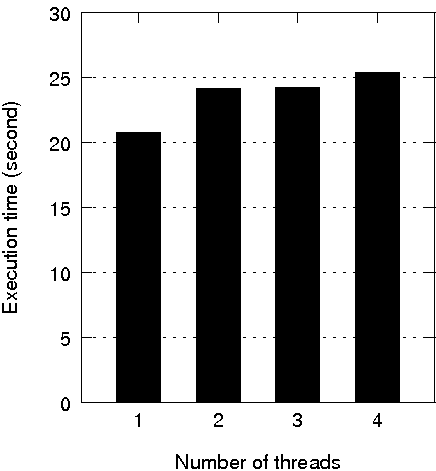
\includegraphics[width=0.4\textwidth]{./Data/numine/original}  	\label{fig:numine:orig} }
   \subfloat[Modified NU-MineBench]{	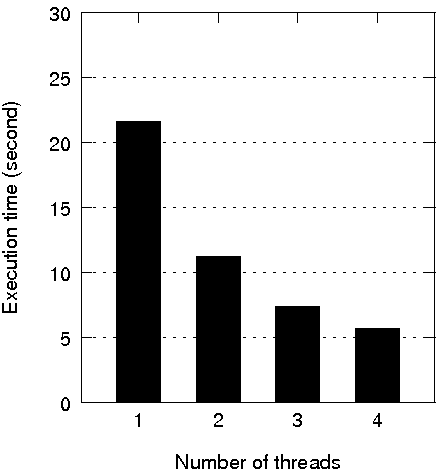
\includegraphics[width=0.4\textwidth]{./Data/numine/modified}  	\label{fig:numine:mod} }
	}
	\caption{Execution times of NU-MineBench based K-means Algorithm \ref{algo:numine} for 100 iterations on Record Linkage Dataset \cite{recordLinkage}, with $K = 2$, $d = 9$, $n = 5749132$. (a) Original NU-MineBench shows slight increase in execution time with increase in thread count due to latencies caused by false sharing. (b) Modified NU-MineBench shows linear speedup with increase in thread count.}
\label{fig:kmean}
\end{figure}


To overcome this shortcoming we ensure that the values stored by each thread occupy distinct cache blocks. We separate every set of $K$ indices inside the array $newClusterSize$ with unused memory locations. We also make similar changes for $newCentroid$ array. This ensures that even for smaller values of $K$ the speedup obtained is linear in thread count; see Figure \ref{fig:numine:mod}. Also, since the size of the cache block is generally small (typically 64 bytes), this change does not make any significant impact on the overall memory requirement.
